\documentclass{article}
\usepackage{graphicx} % Required for inserting images
\usepackage [utf8]{ctex}
\usepackage{listings}

\title{hadoop-wordcount}
\author{211870287 丁旭 }
\date{September 2023}

\begin{document}

\maketitle

\section{hadoop环境配置}
\begin{enumerate}

    \item 远程连接ECS实例
        \par 
        \begin{figure}[htp]
            \centering
            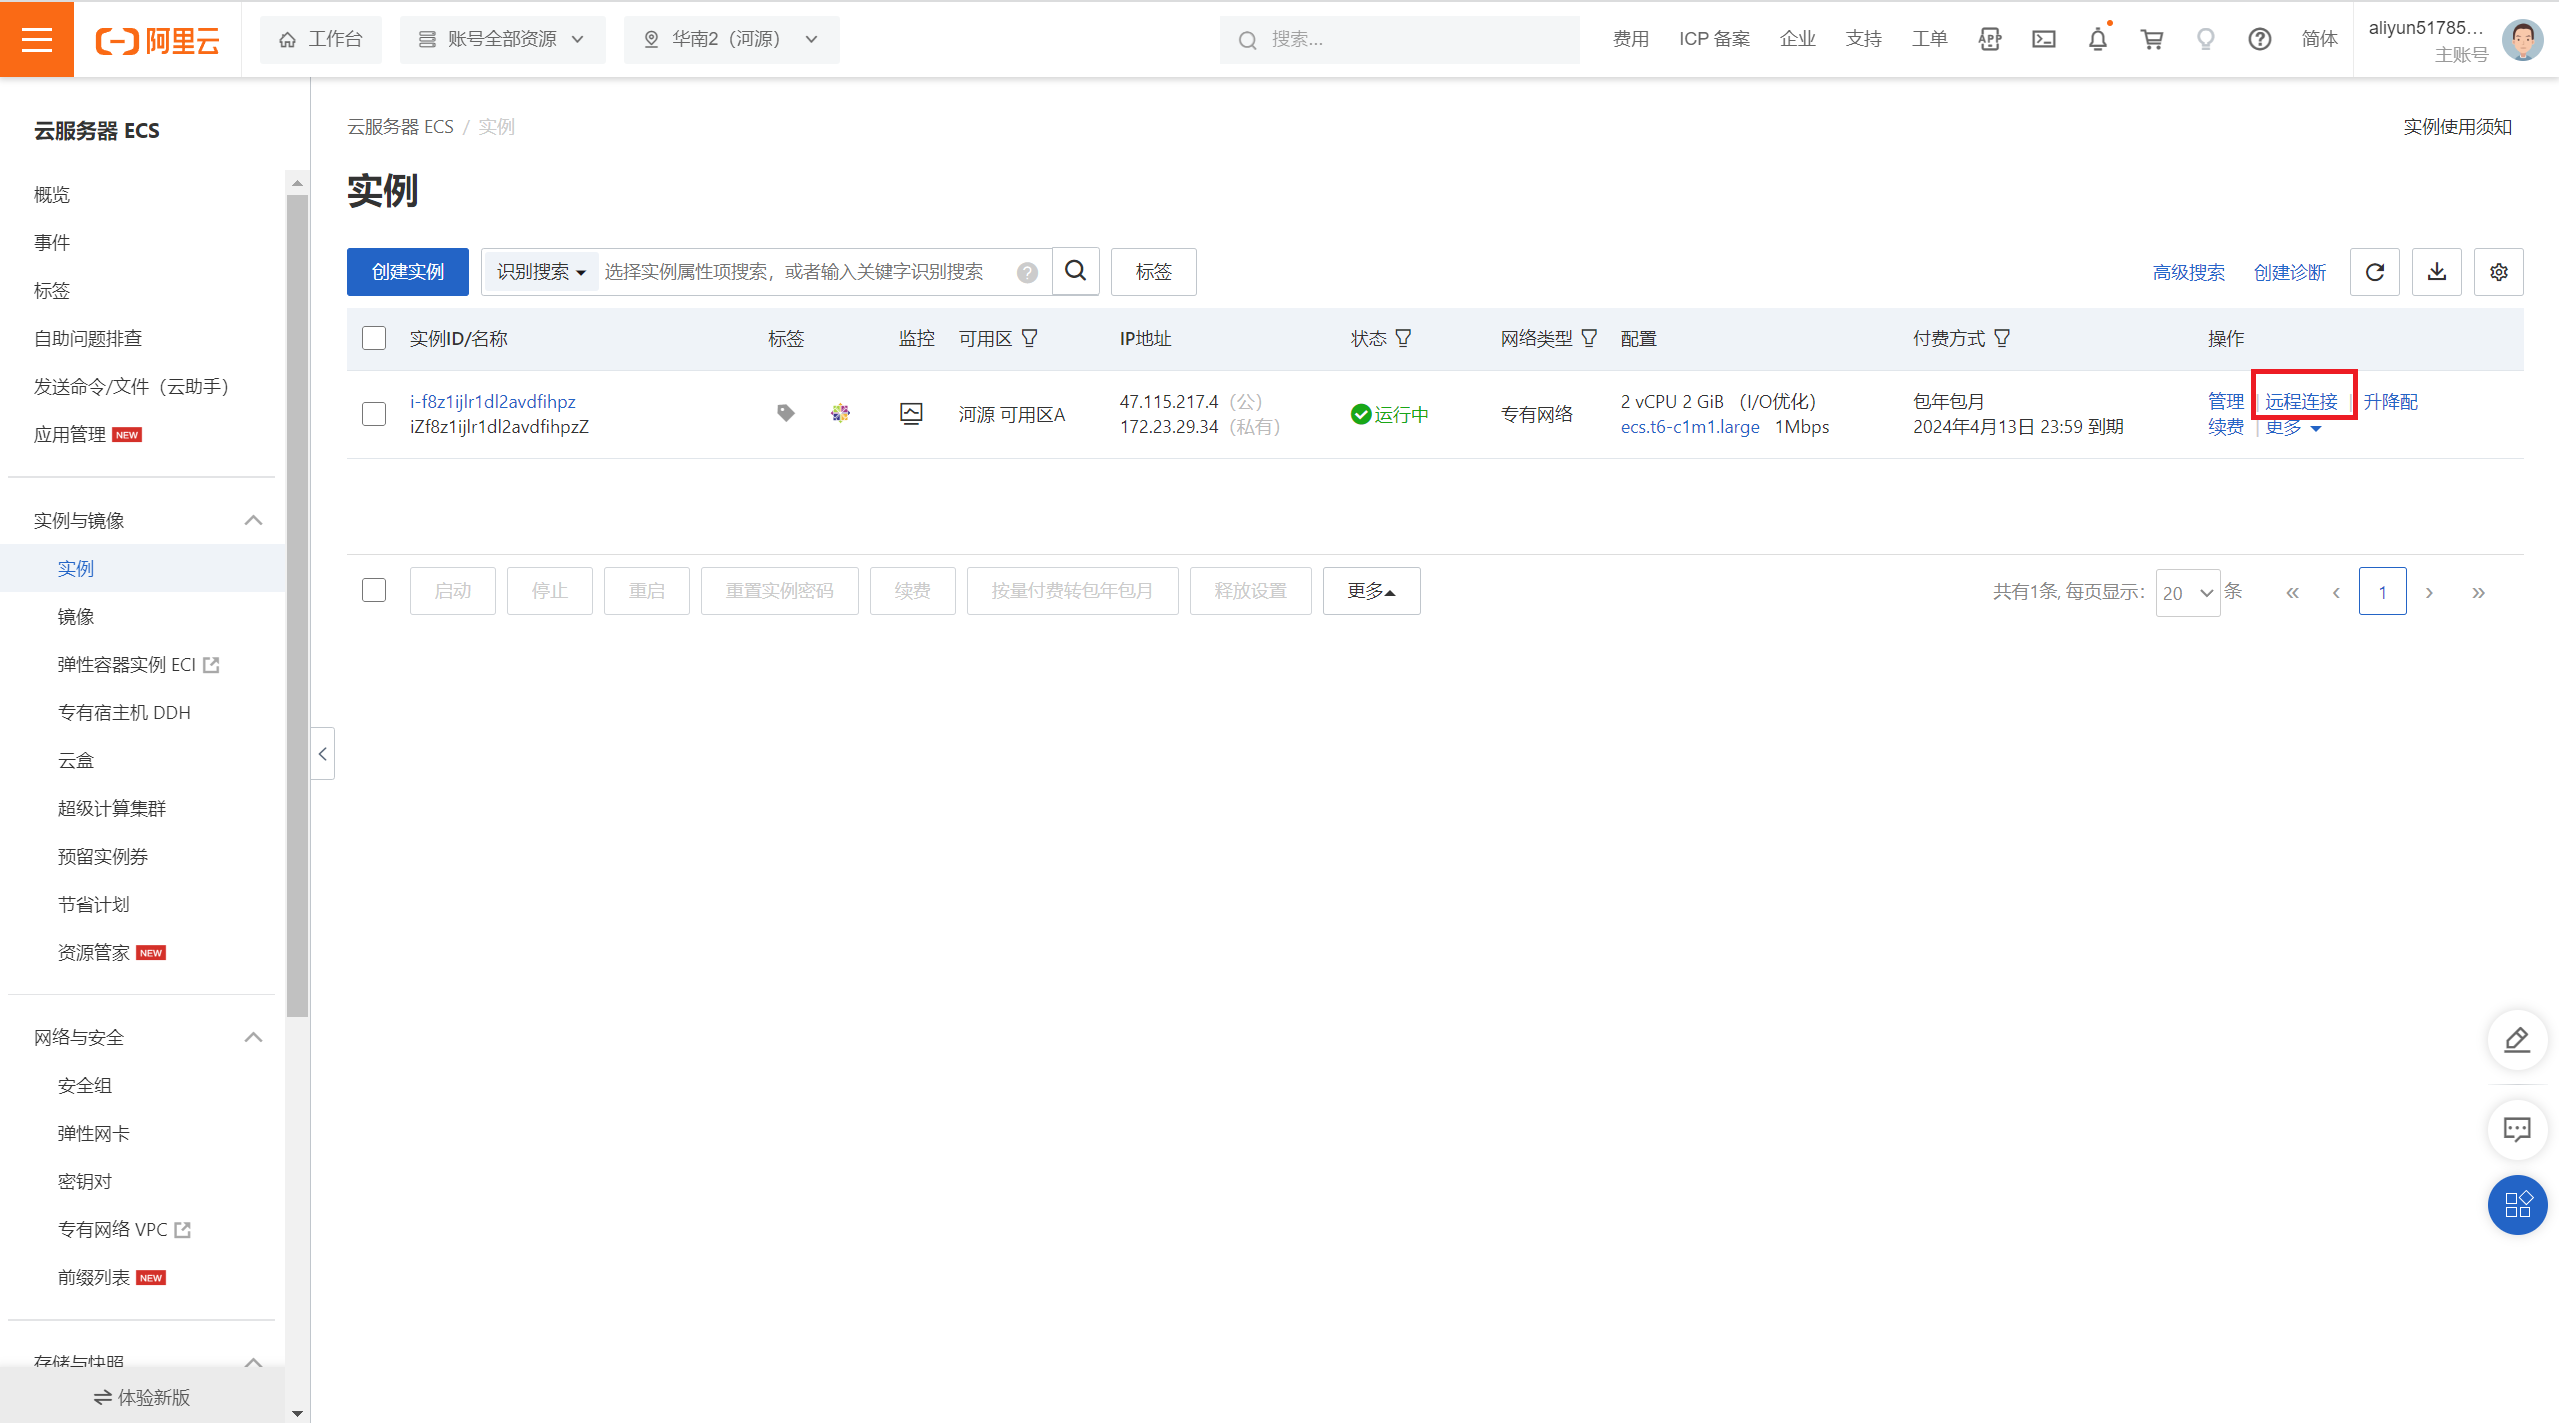
\includegraphics[width=15cm]{远程连接}
            \caption{云服务器控制台界面}
            \label{fig:galaxy}
        \end{figure}
    \item 安装jdk1.8

        \begin{enumerate}
            \item 下载JDK安装包
            
            \begin{lstlisting}
wget https://download.java.net/openjdk/jdk8u41/ri/ 
(接)openjdk-8u41-b04-linux-x64-14_jan_2020.tar.gz
            \end{lstlisting}
            \item 解压JDK安装包
            
            \begin{lstlisting}
tar -zxvf openjdk-8u41-b04-linux-x64-14_jan_2020.tar.gz
            \end{lstlisting}
            \item 移动并重命名JDK安装包
            
            \begin{lstlisting}
mv java-se-8u41-ri/ /usr/java8
            \end{lstlisting}
            \item 配置java环境
            
            \begin{lstlisting}
echo 'export JAVA_HOME=/usr/java8' >> /etc/profile
echo 'export PATH=$PATH:$JAVA_HOME/bin' >> /etc/profile
source /etc/profile
            \end{lstlisting}

            \item 查看java是否安装
            \begin{figure}[htp]
                \centering
                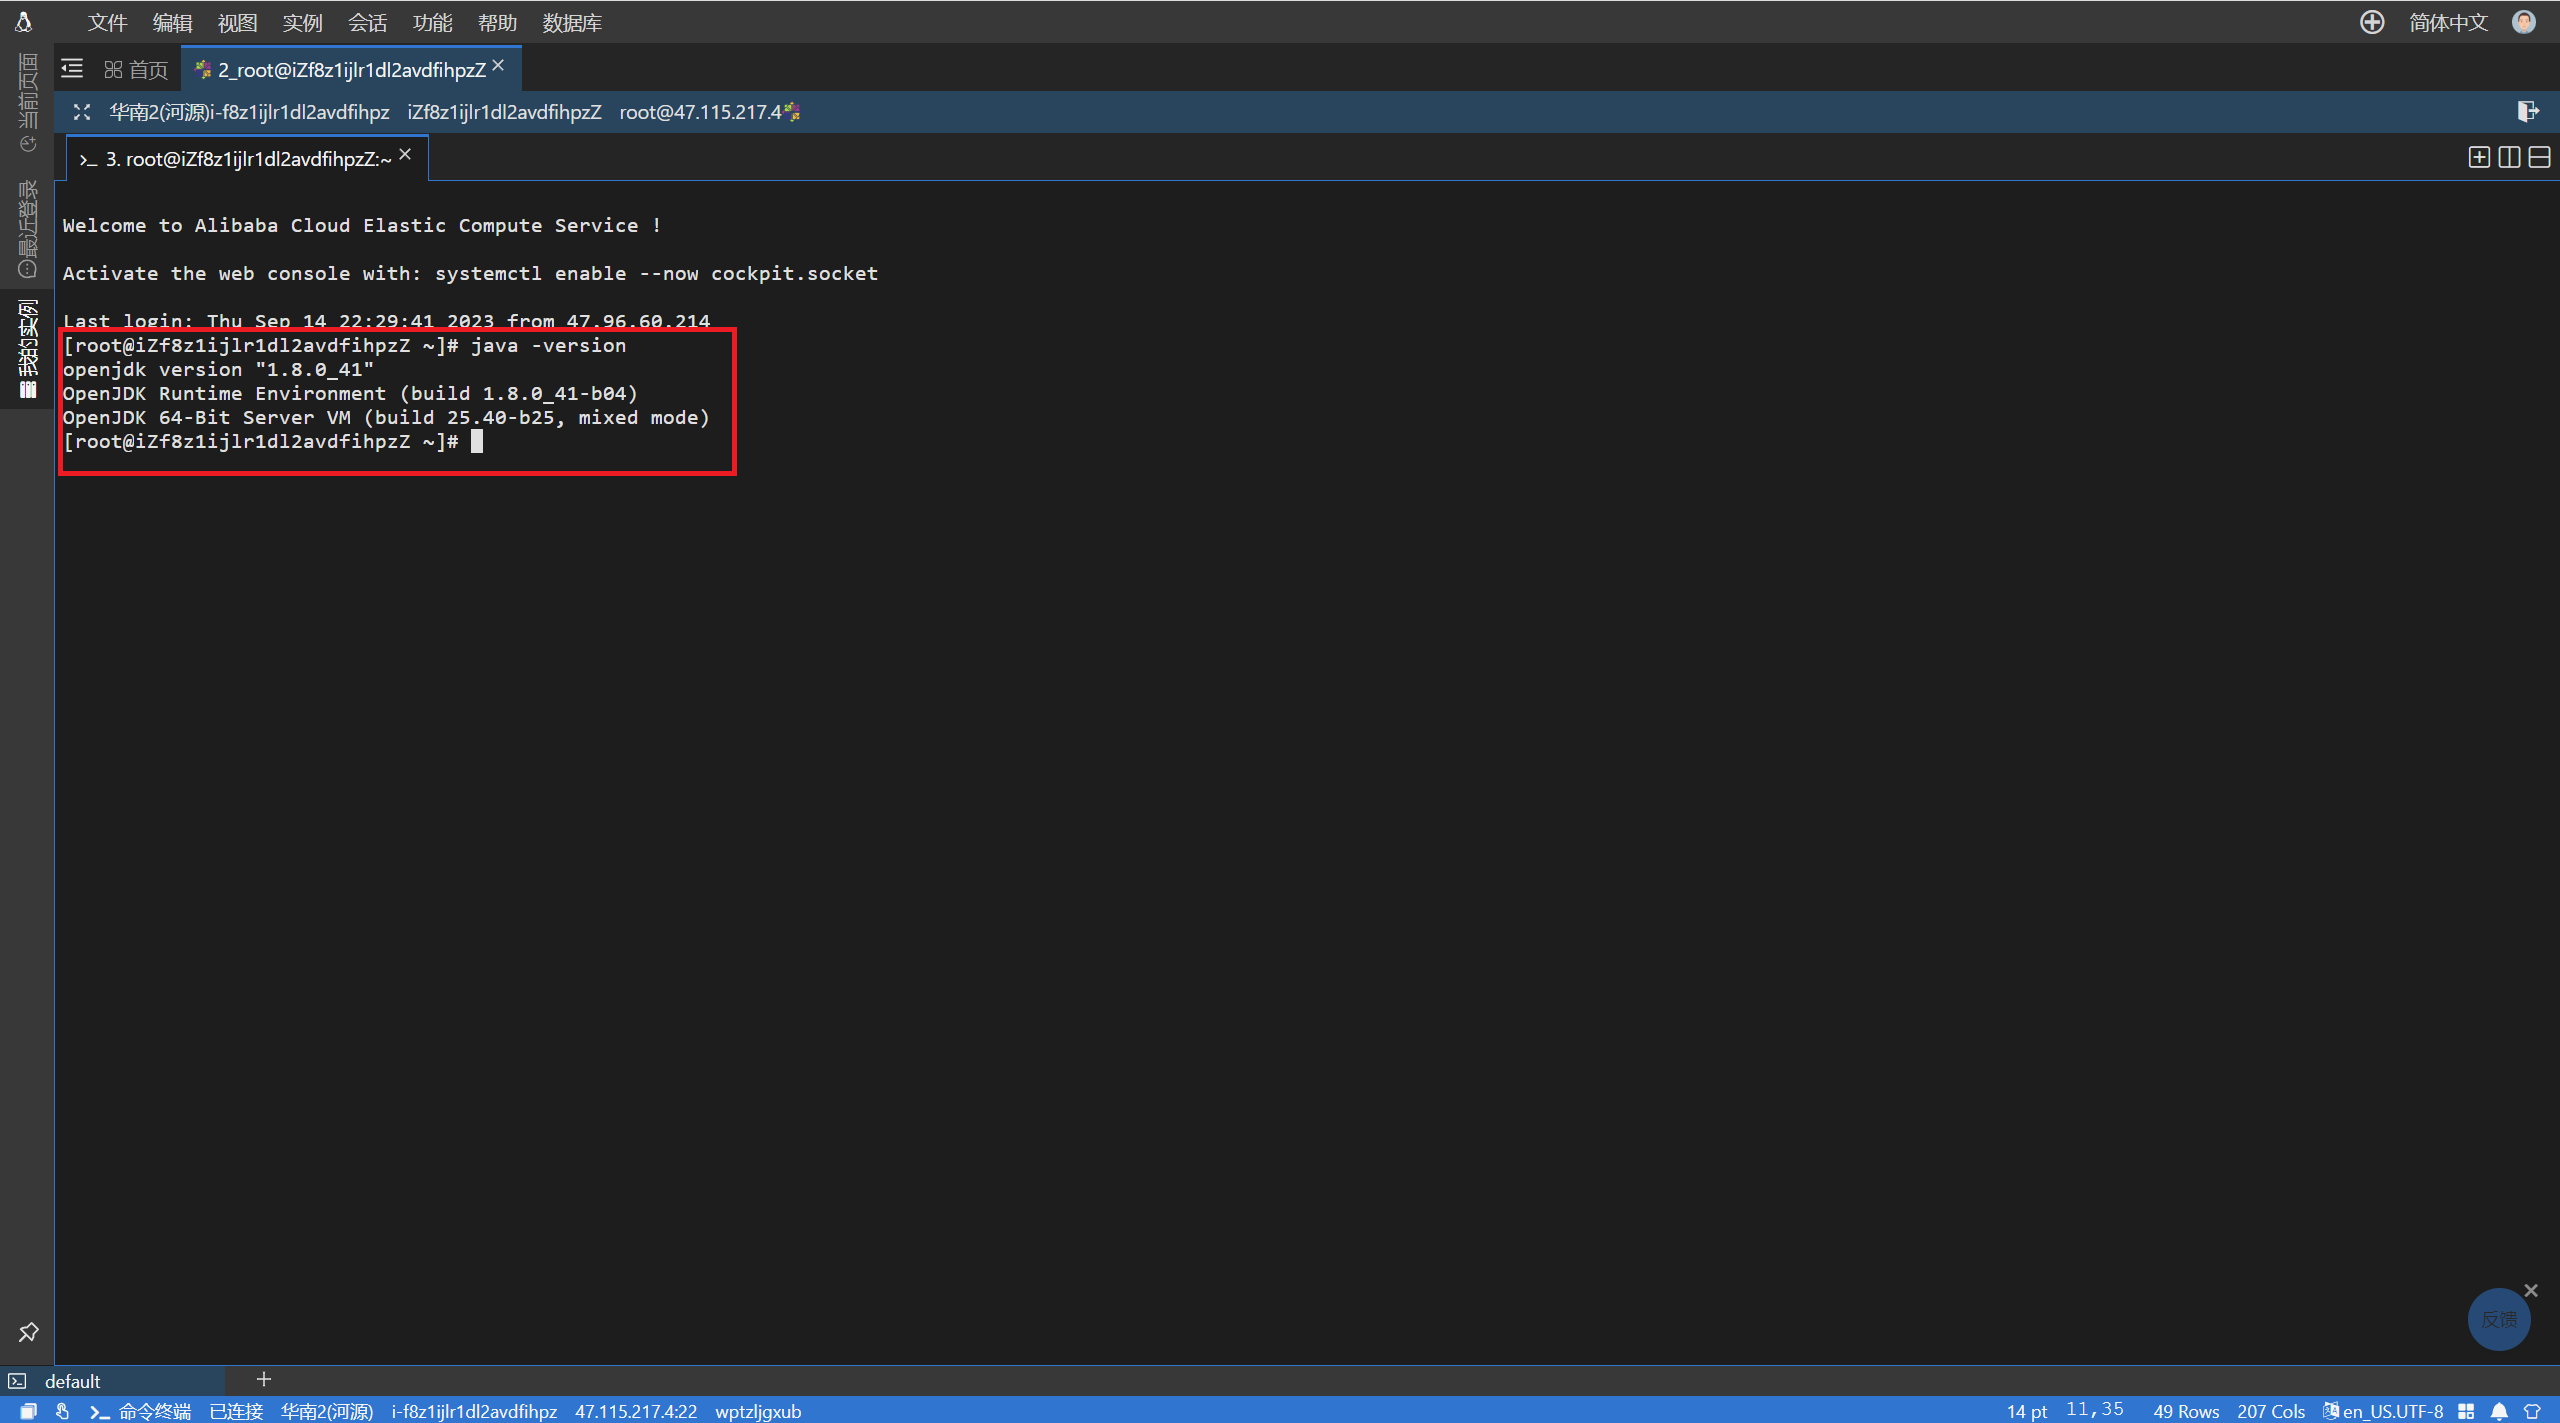
\includegraphics[width=15cm]{java安装验证}
                \caption{java验证: java -version}
                \label{fig:gala}
            \end{figure}
        \end{enumerate}
    
    \item 安装Hadoop
        \begin{enumerate}
            \item 下载Hadoop安装包            
            \begin{lstlisting}
wget https://mirrors.bfsu.edu.cn/apache/hadoop/common/hadoop-2.10.1/hadoop-(接)2.10.1.tar.gz
            \end{lstlisting}

            \item 解压Hadoop安装包至/opt/hadoop
            \begin{lstlisting}
tar -zxvf hadoop-2.10.1.tar.gz -C /opt/
mv /opt/hadoop-2.10.1 /opt/hadoop
            \end{lstlisting}

            \item 配置Hadoop环境变量
            \begin{lstlisting}
echo 'export HADOOP_HOME=/opt/hadoop/' >> /etc/profile
echo 'export PATH=$PATH:$HADOOP_HOME/bin' >> /etc/profile
echo 'export PATH=$PATH:$HADOOP_HOME/sbin' >> /etc/profile
source /etc/profile    
            \end{lstlisting}

            \item 修改配置文件yarn-env.sh和hadoop-env.sh
            \begin{lstlisting}
echo "export JAVA_HOME=/usr/java8" >> 
/opt/hadoop/etc/hadoop/yarn-env.sh

echo "export JAVA_HOME=/usr/java8" >> 
/opt/hadoop/etc/hadoop/hadoop-env.sh  
            \end{lstlisting}

            \item 验证Hadoop是否安装成功
            \begin{figure}[htp]
                \centering
                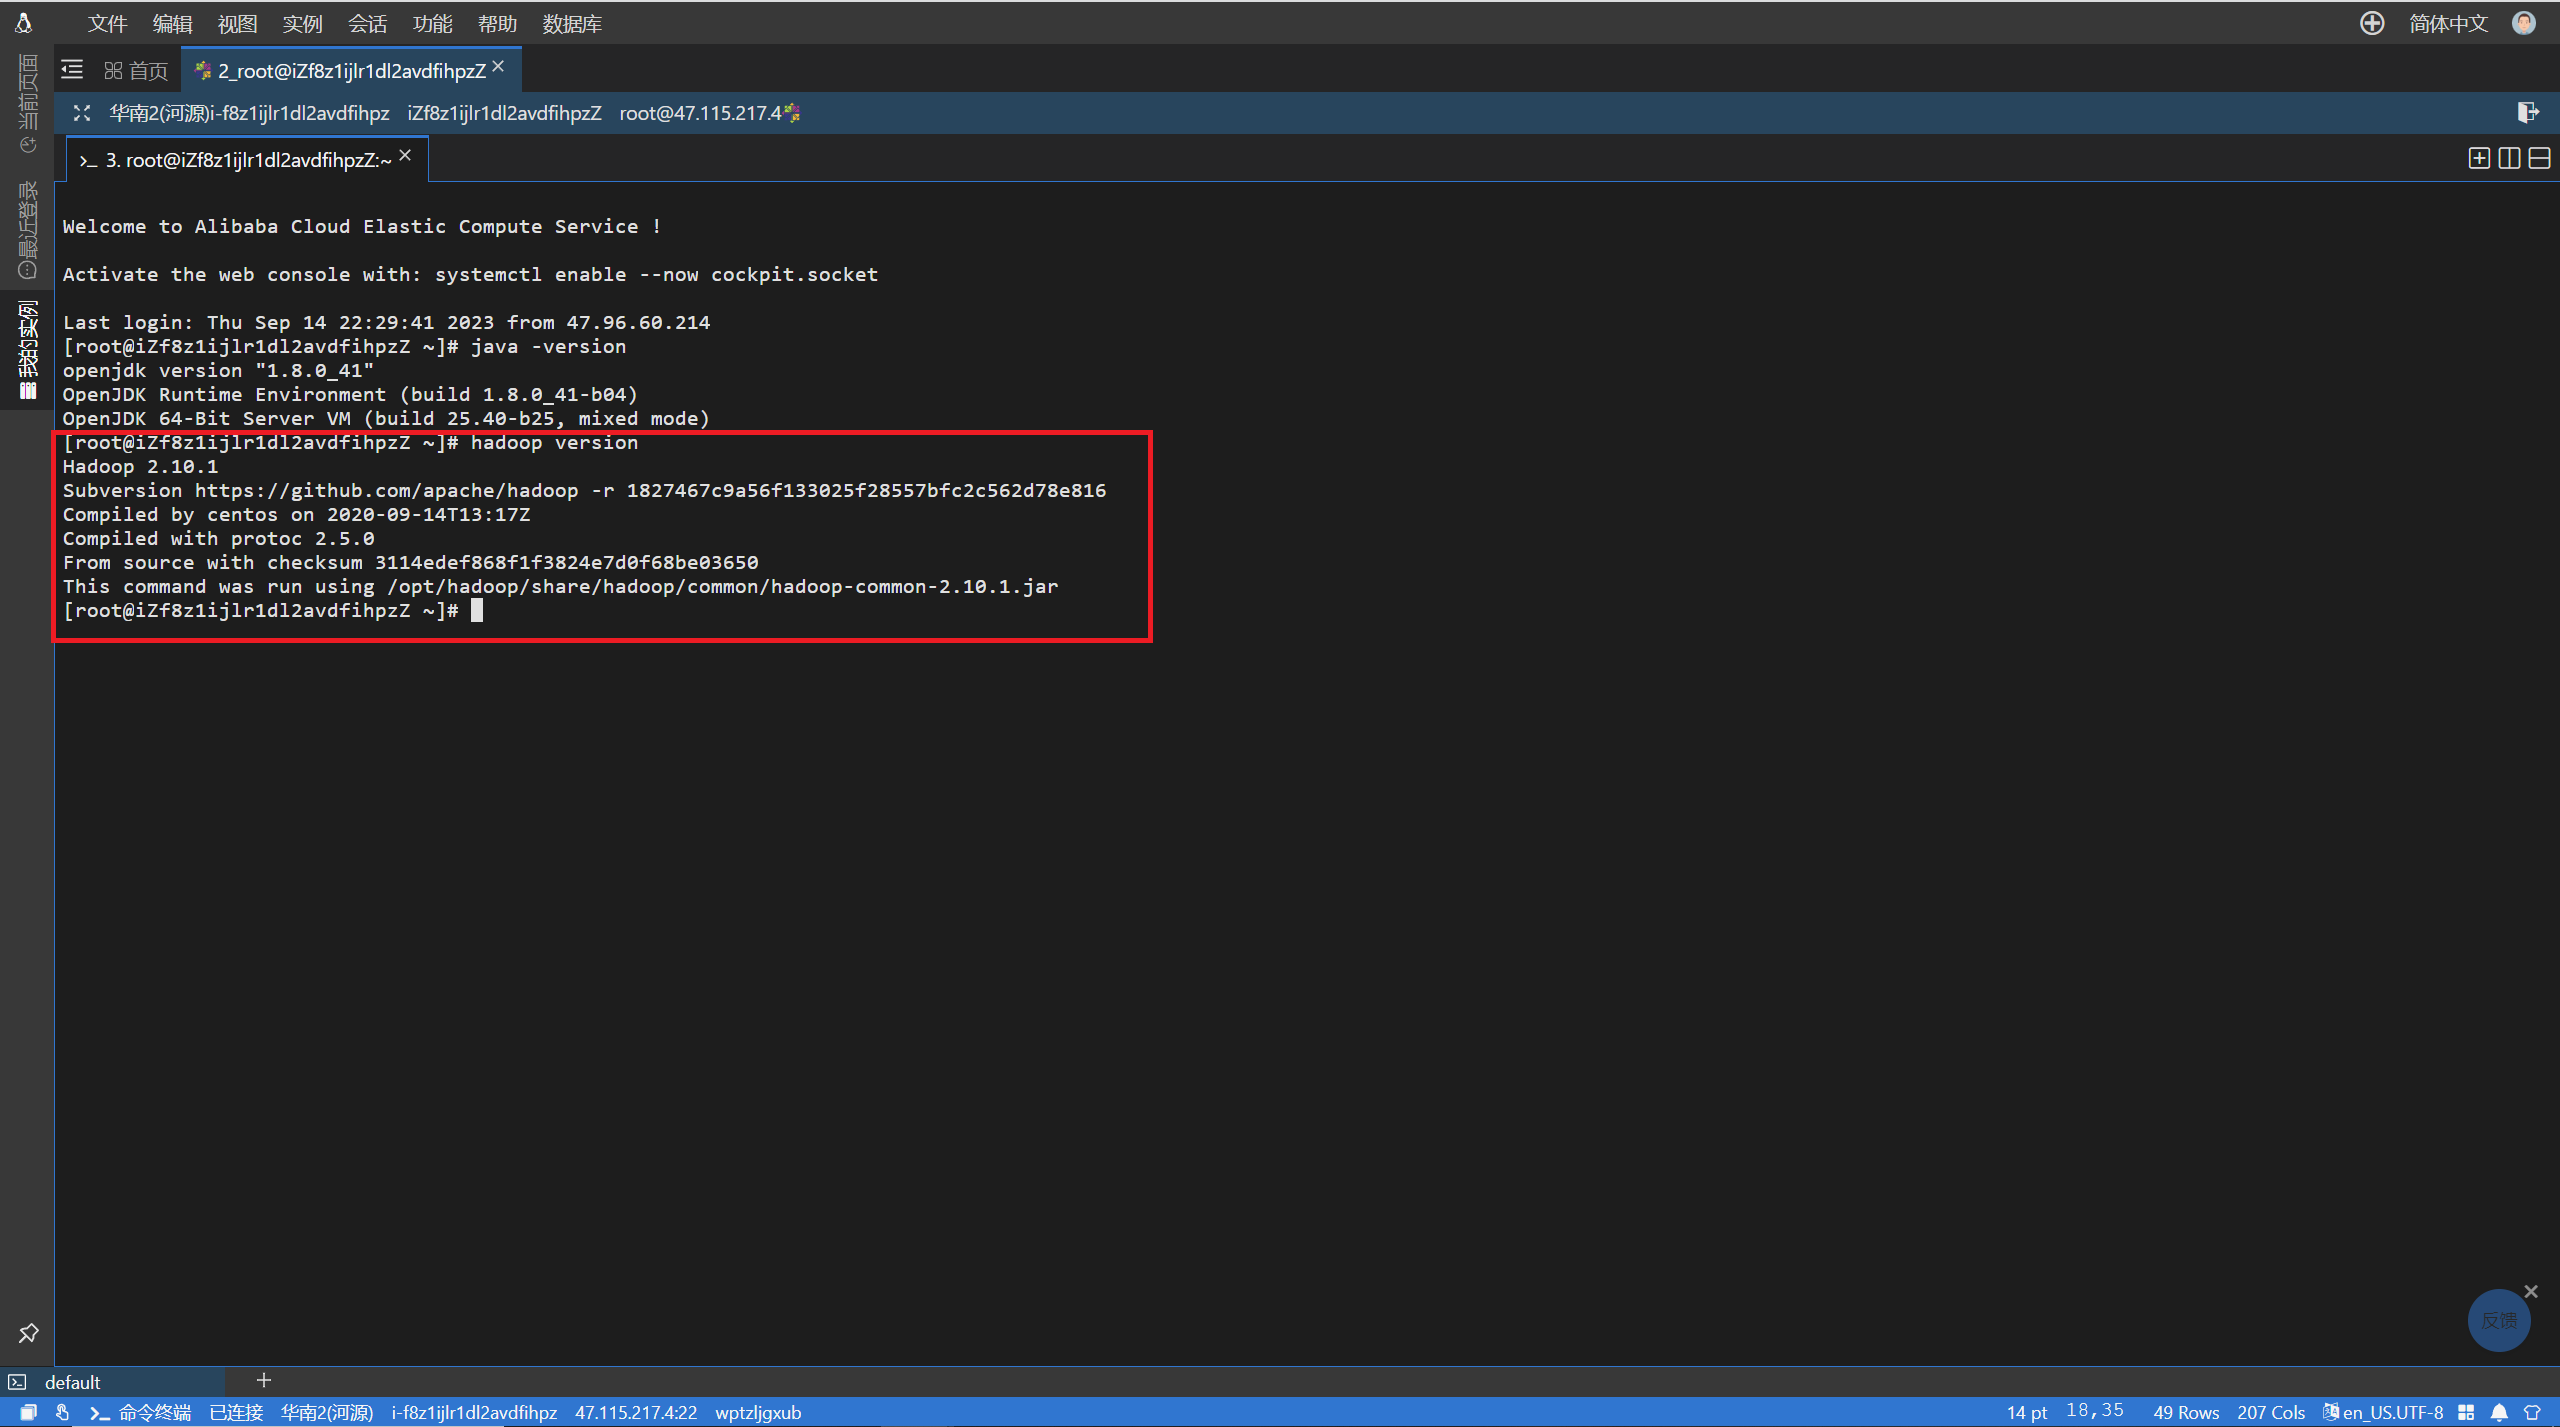
\includegraphics[width=10cm]{hadoop安装验证}
                \caption{hadoop安装验证}
                \label{fig:gaa}
            \end{figure}
            
        \end{enumerate}
    \item 配置Hadoop
        
        \begin{lstlisting}
进入编辑界面
vim /opt/hadoop/etc/hadoop/core-site.xml
        \end{lstlisting}
    
        \begin{lstlisting}
在<configuration></configuration>节点内,插入如下内容。
<property>
    <name>hadoop.tmp.dir</name>
    <value>file:/opt/hadoop/tmp</value>
    <description>location to store temporary files</description>
</property>
<property>
    <name>fs.defaultFS</name>
    <value>hdfs://localhost:9000</value>
</property>
        \end{lstlisting}

        \begin{lstlisting}
进入编辑界面
vim /opt/hadoop/etc/hadoop/hdfs-site.xml
        \end{lstlisting}
    
        \begin{lstlisting}
在<configuration></configuration>节点内,插入如下内容
<property>
    <name>dfs.replication</name>
    <value>1</value>
</property>
<property>
    <name>dfs.namenode.name.dir</name>
    <value>file:/opt/hadoop/tmp/dfs/name</value>
</property>
<property>
    <name>dfs.datanode.data.dir</name>
    <value>file:/opt/hadoop/tmp/dfs/data</value>
</property>
        \end{lstlisting}
    \item 配置SSH免密登录
    \begin{lstlisting}
创建公钥和私钥
ssh-keygen -t rsa
    \end{lstlisting}
    \begin{lstlisting}
执行以下命令,将公钥添加到authorized_keys文件中
cd .ssh
cat id_rsa.pub >> authorized_keys
    \end{lstlisting}
    
\end{enumerate}
\section{启动hadoop}
\begin{enumerate}
    \item 执行以下命令,初始化namenode
    \begin{lstlisting}
hadoop namenode -format
    \end{lstlisting}
    \item 依次执行以下命令,启动Hadoop
    \begin{lstlisting}
start-dfs.sh
start-yarn.sh
    \end{lstlisting}
    \item 查看成功启动的进程
    \begin{figure}[htp]
        \centering
        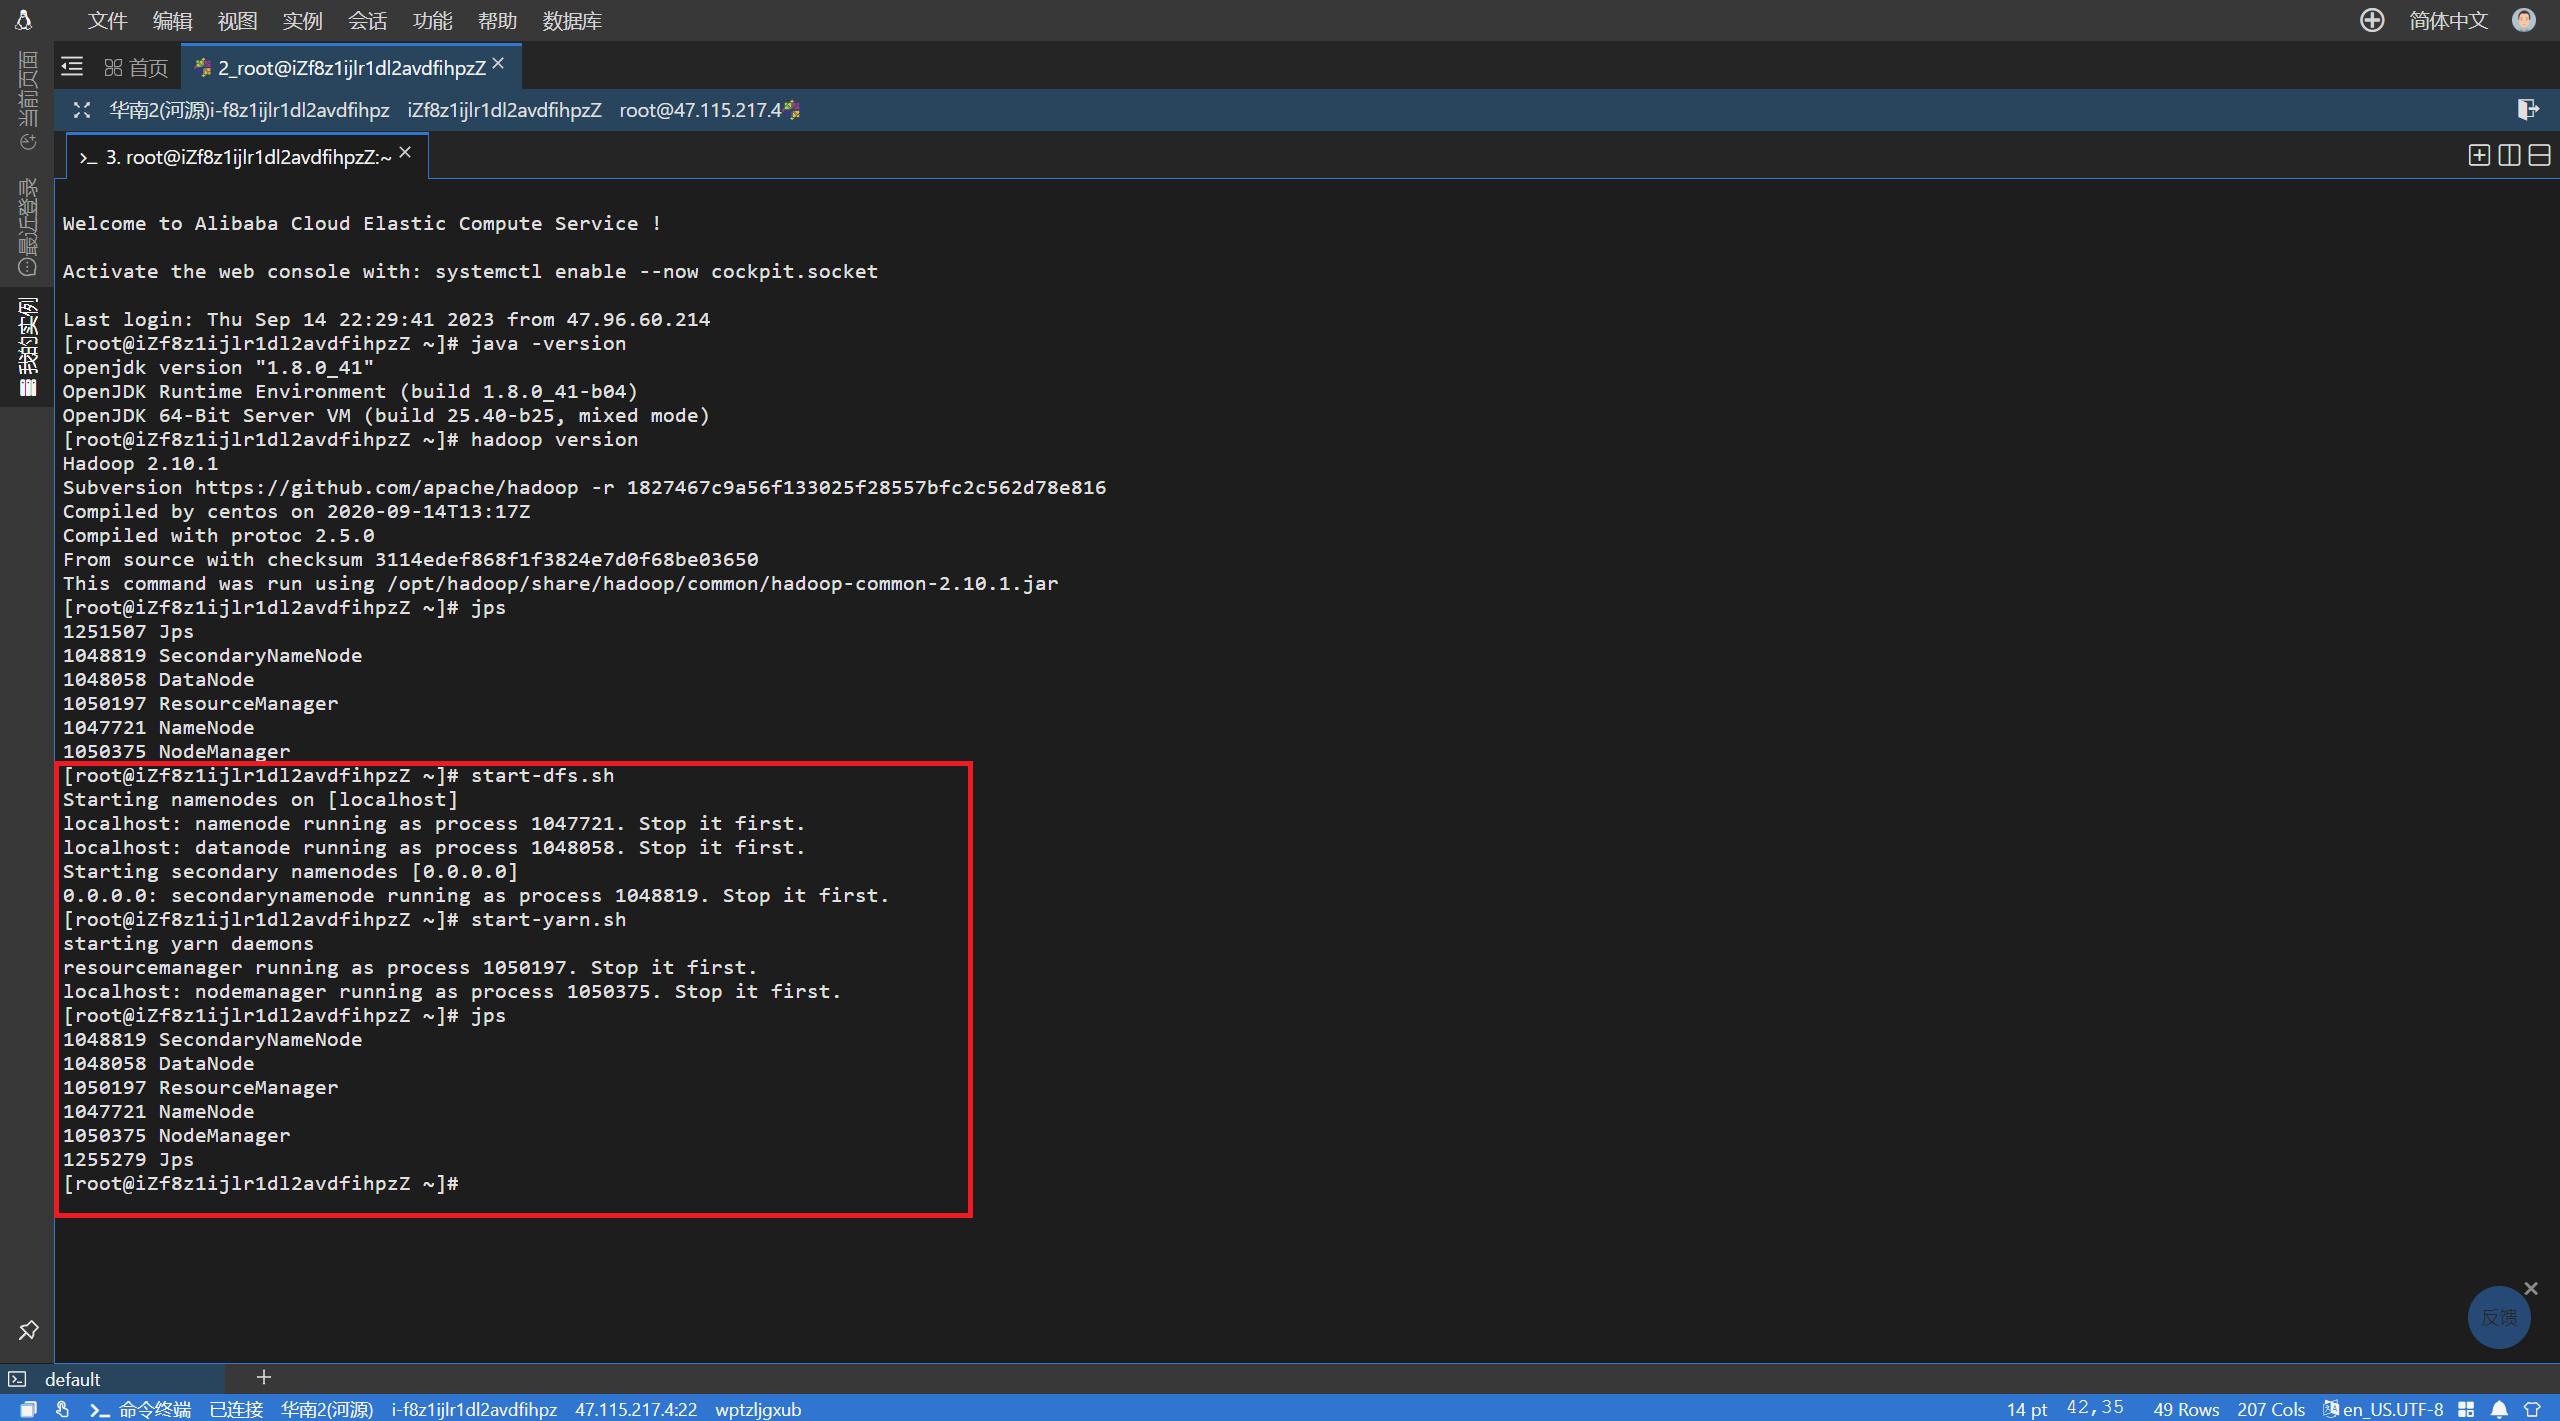
\includegraphics[width=10cm]{hadoop启动验证}
        \caption{hadoop启动验证}
        \label{fig:aa}
    \end{figure}
    \item 打开浏览器访问http://<ECS公网IP>:8088和http://<ECS公网IP>:50070
    \newpage
    \begin{figure}[htp]
        \centering
        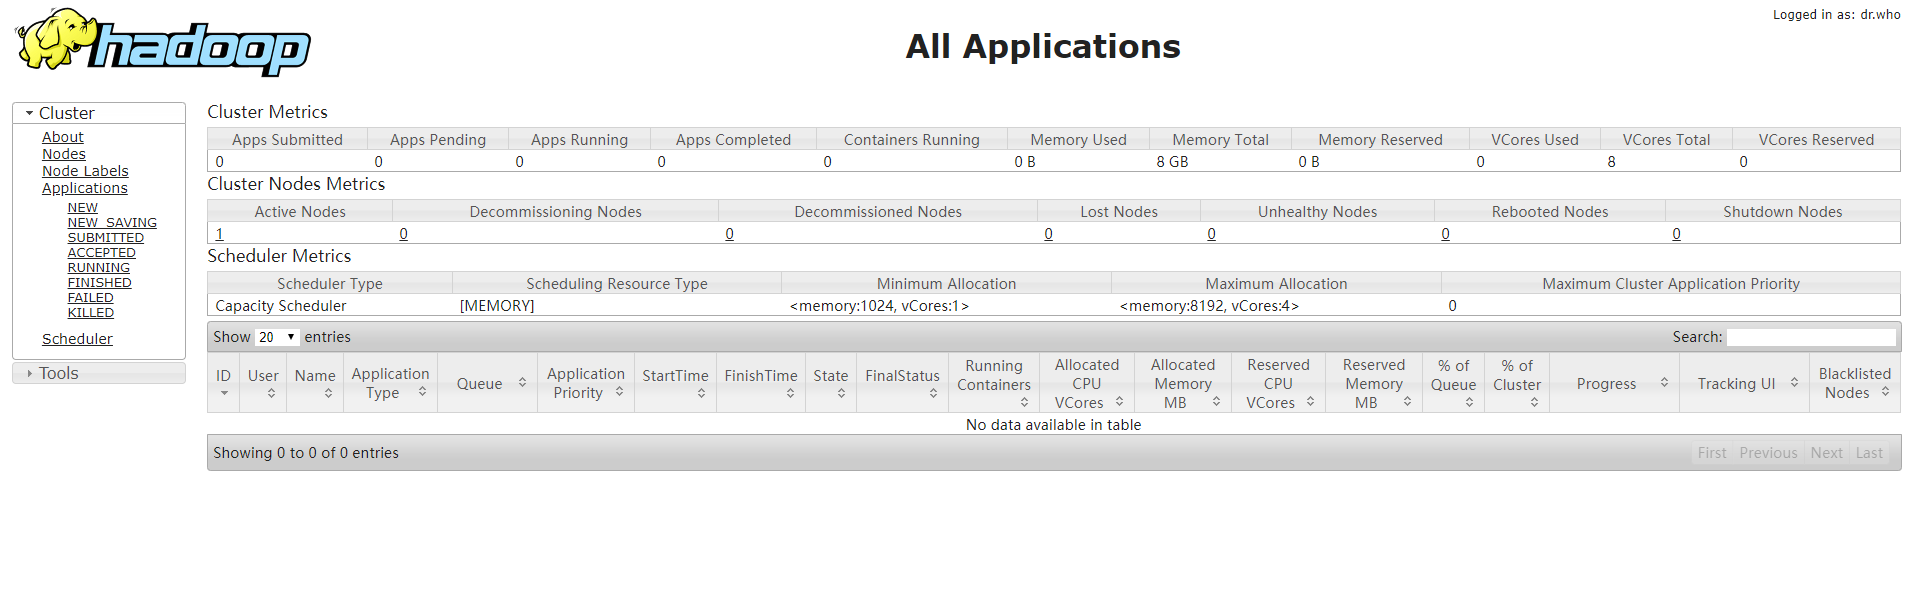
\includegraphics[width=10cm]{8088port}
        \caption{http://<ECS公网IP>:8088}
        \label{fig:aa}
    \end{figure}
    \begin{figure}[htp]
        \centering
        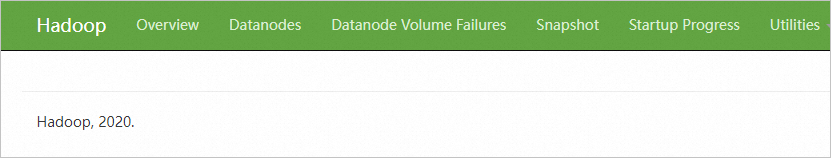
\includegraphics[width=10cm]{50070port}
        \caption{http://<ECS公网IP>:50070}
        \label{fig:aa}
    \end{figure}
\end{enumerate}
\section{scala环境配置}
\begin{enumerate}
    \item 进入到/usr/local/share文件夹
    \begin{lstlisting}
cd /usr/local/share
    \end{lstlisting}

    \item 安装包下载
    \begin{lstlisting}
wget https://downloads.lightbend.com/scala/2.12.6/scala-2.12.6.tgz
    \end{lstlisting}

    \item 解压文件
    \begin{lstlisting}
tar -xvzf scala-2.12.6.tgz
    \end{lstlisting}

    \item 添加环境变量
    \begin{lstlisting}
vim /etc/profile
export PATH="$PATH:/usr/local/share/scala-2.12.6/bin"
source /etc/profile
    \end{lstlisting}

    \item scala环境检验
    \begin{figure}[htp]
        \centering
        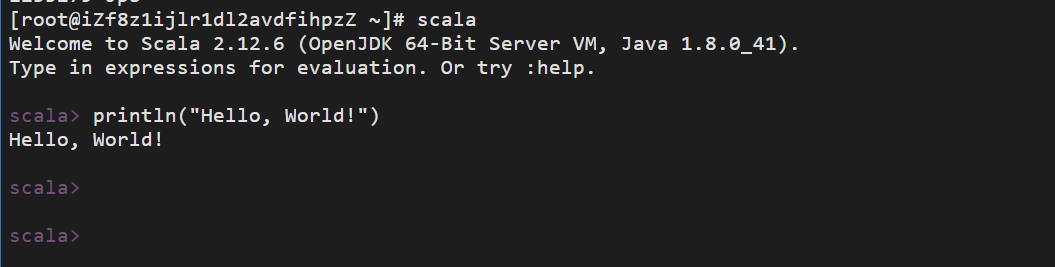
\includegraphics[width=10cm]{scala环境检验}
        \caption{scala: hello,world!}
        \label{fig:aa}
    \end{figure}
    
    
    
\end{enumerate}

\section{在hadoop环境下编写scala的wordcount}
\begin{enumerate}
    \item 启动hadoop
    \begin{lstlisting}
cd /usr/hadoop/hadoop-2.6.2/
sbin/start-dfs.sh
sbin/start-yarn.sh
    \end{lstlisting}

    \item 创建本地数据文件
    \begin{lstlisting}
cd ~/
mkdir ~/file
cd file
echo "Hello World , welcome to Big Data Analysis" > test1.txt
echo "Big Data Analysis is a good lesson " > test2.txt
    \end{lstlisting}

    \item 创建scala代码
    \begin{lstlisting}
import java.io.File
import scala.io.Source
object WordCount {
  def main(args: Array[String]): Unit = {
    val dirfile=new File(args(0))
    val files=dirfile.listFiles
    for(file <- files) println(file)
    val listFiles=files.toList
    val wordsMap=scala.collection.mutable.Map[String,Int]()
    listFiles.foreach( file =>Source.fromFile(file).getLines().
    foreach(line=>line.split(" ").
                  foreach(
                      word=>{
                        if (wordsMap.contains(word)) {
                          wordsMap(word)+=1
                        }else {
                          wordsMap+=(word->1)
                        }
                      }
                  )
            )

    )
    println(wordsMap)
    for((key,value)<-wordsMap) println(key+": "+value)
  }
}
    \end{lstlisting}
    \item 将数据文件传到HDFS的input目录下
    \begin{lstlisting}
hadoop fs -mkdir /input
hadoop fs -put ~/file/test*.txt /input
sbin/start-yarn.sh
    \end{lstlisting}
    \item 运行程序
    \begin{lstlisting}
    第一种运行方式
hadoop jar /opt/hadoop/share/hadoop/mapreduce/hadoop-mapreduce
-examples-2.10.1.jar wordcount /input /output

    第二种运行方式
编写build.sh
#!/bin/bash

# 设置输出 Jar 文件的名称
JAR_NAME="WordCount.jar"

# 编译 Scala 文件
scalac WordCount.scala

# 创建临时目录并将编译生成的 .class 文件复制到该目录中
mkdir tmp
find . -name '*.class' -exec cp {} tmp/ \;

# 创建空的 MANIFEST.MF 文件
touch MANIFEST.MF

# 在 MANIFEST.MF 文件中写入主类的信息,替换 "com.example.MainClass" 为你的主类的完整名称
echo "Main-Class: WordCount" >> MANIFEST.MF

# 打包 .class 文件和 MANIFEST.MF 文件为 Jar 文件
jar cfm $JAR_NAME MANIFEST.MF -C tmp .

# 删除临时目录和 MANIFEST.MF 文件
rm -rf tmp MANIFEST.MF

运行build.sh
sh build.sh
配置hadoop的scala环境
export HADOOP_CLASSPATH=$HADOOP_CLASSPATH:/usr/local/share
/scala-2.12.6/lib/*
source ~/.bashrc

在hadoop环境运行scala的jar包
hadoop jar /root/wordcount/WordCount.jar /root/file
    \end{lstlisting}
    \begin{figure}[htp]
        \centering
        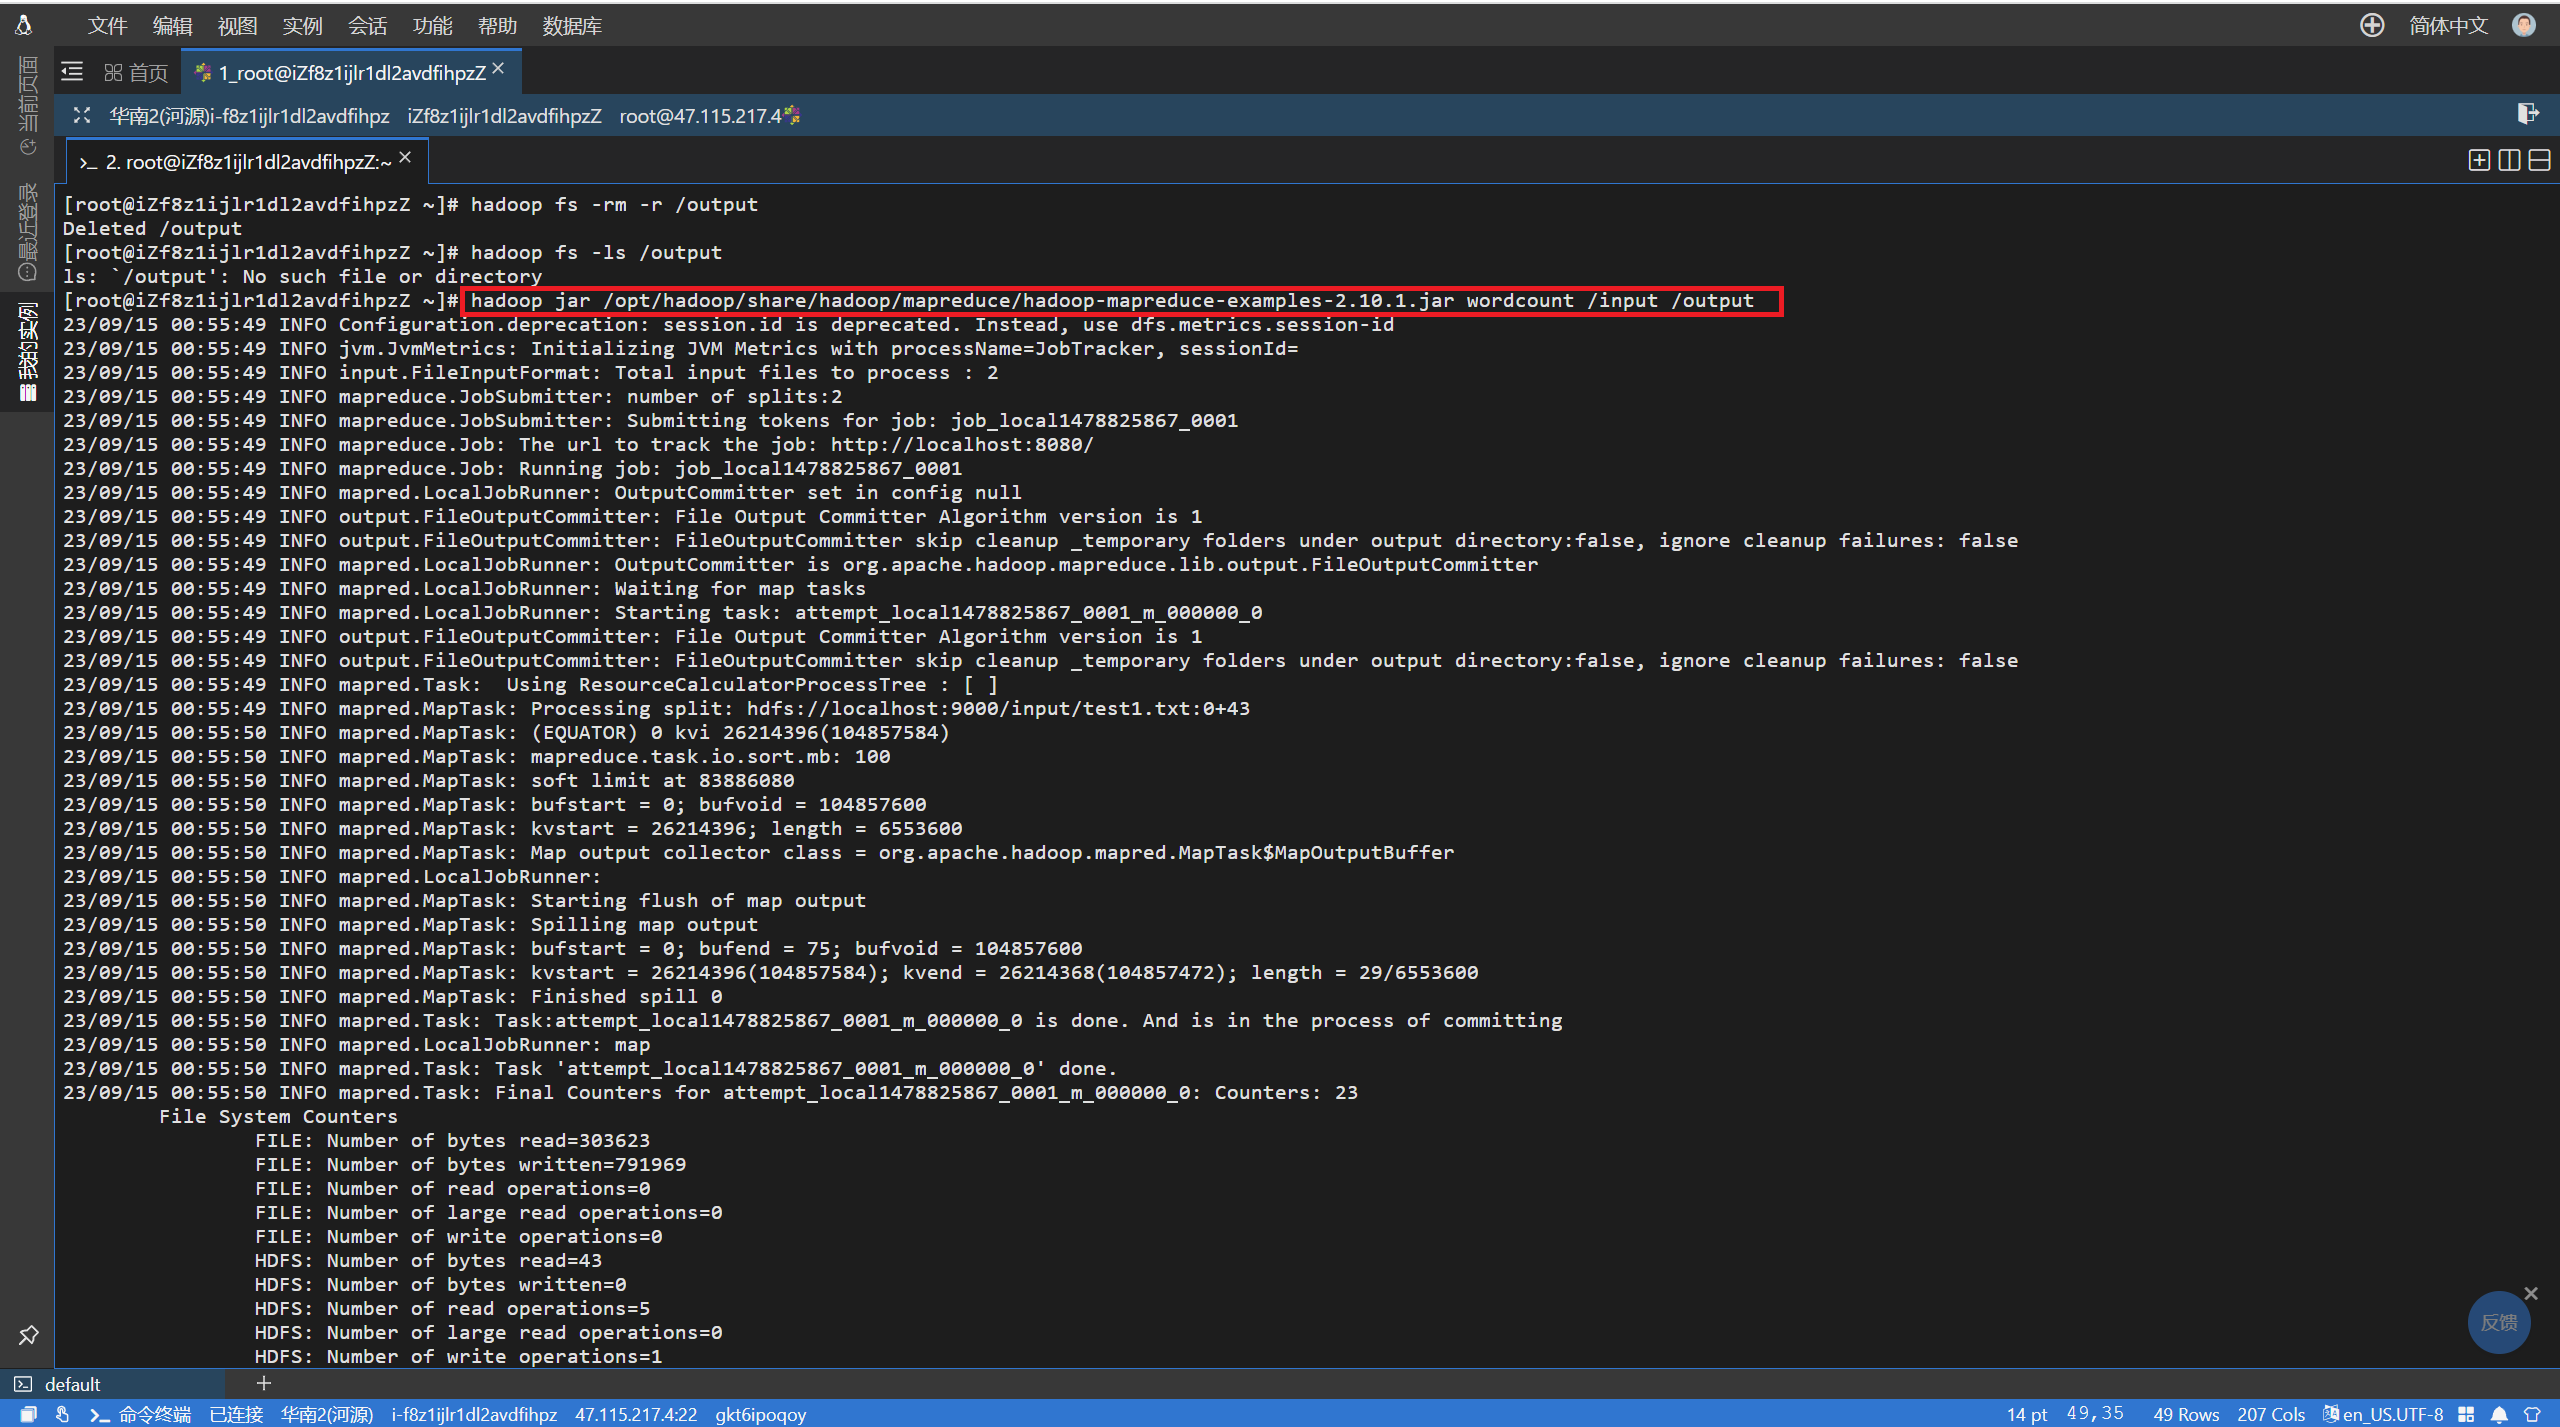
\includegraphics[width=10cm]{运行.png}
        \caption{第一种方式在hadoop环境下,运行scala的wordcount}
        \label{fi:a}
    \end{figure}
    \begin{figure}[htp]
        \centering
        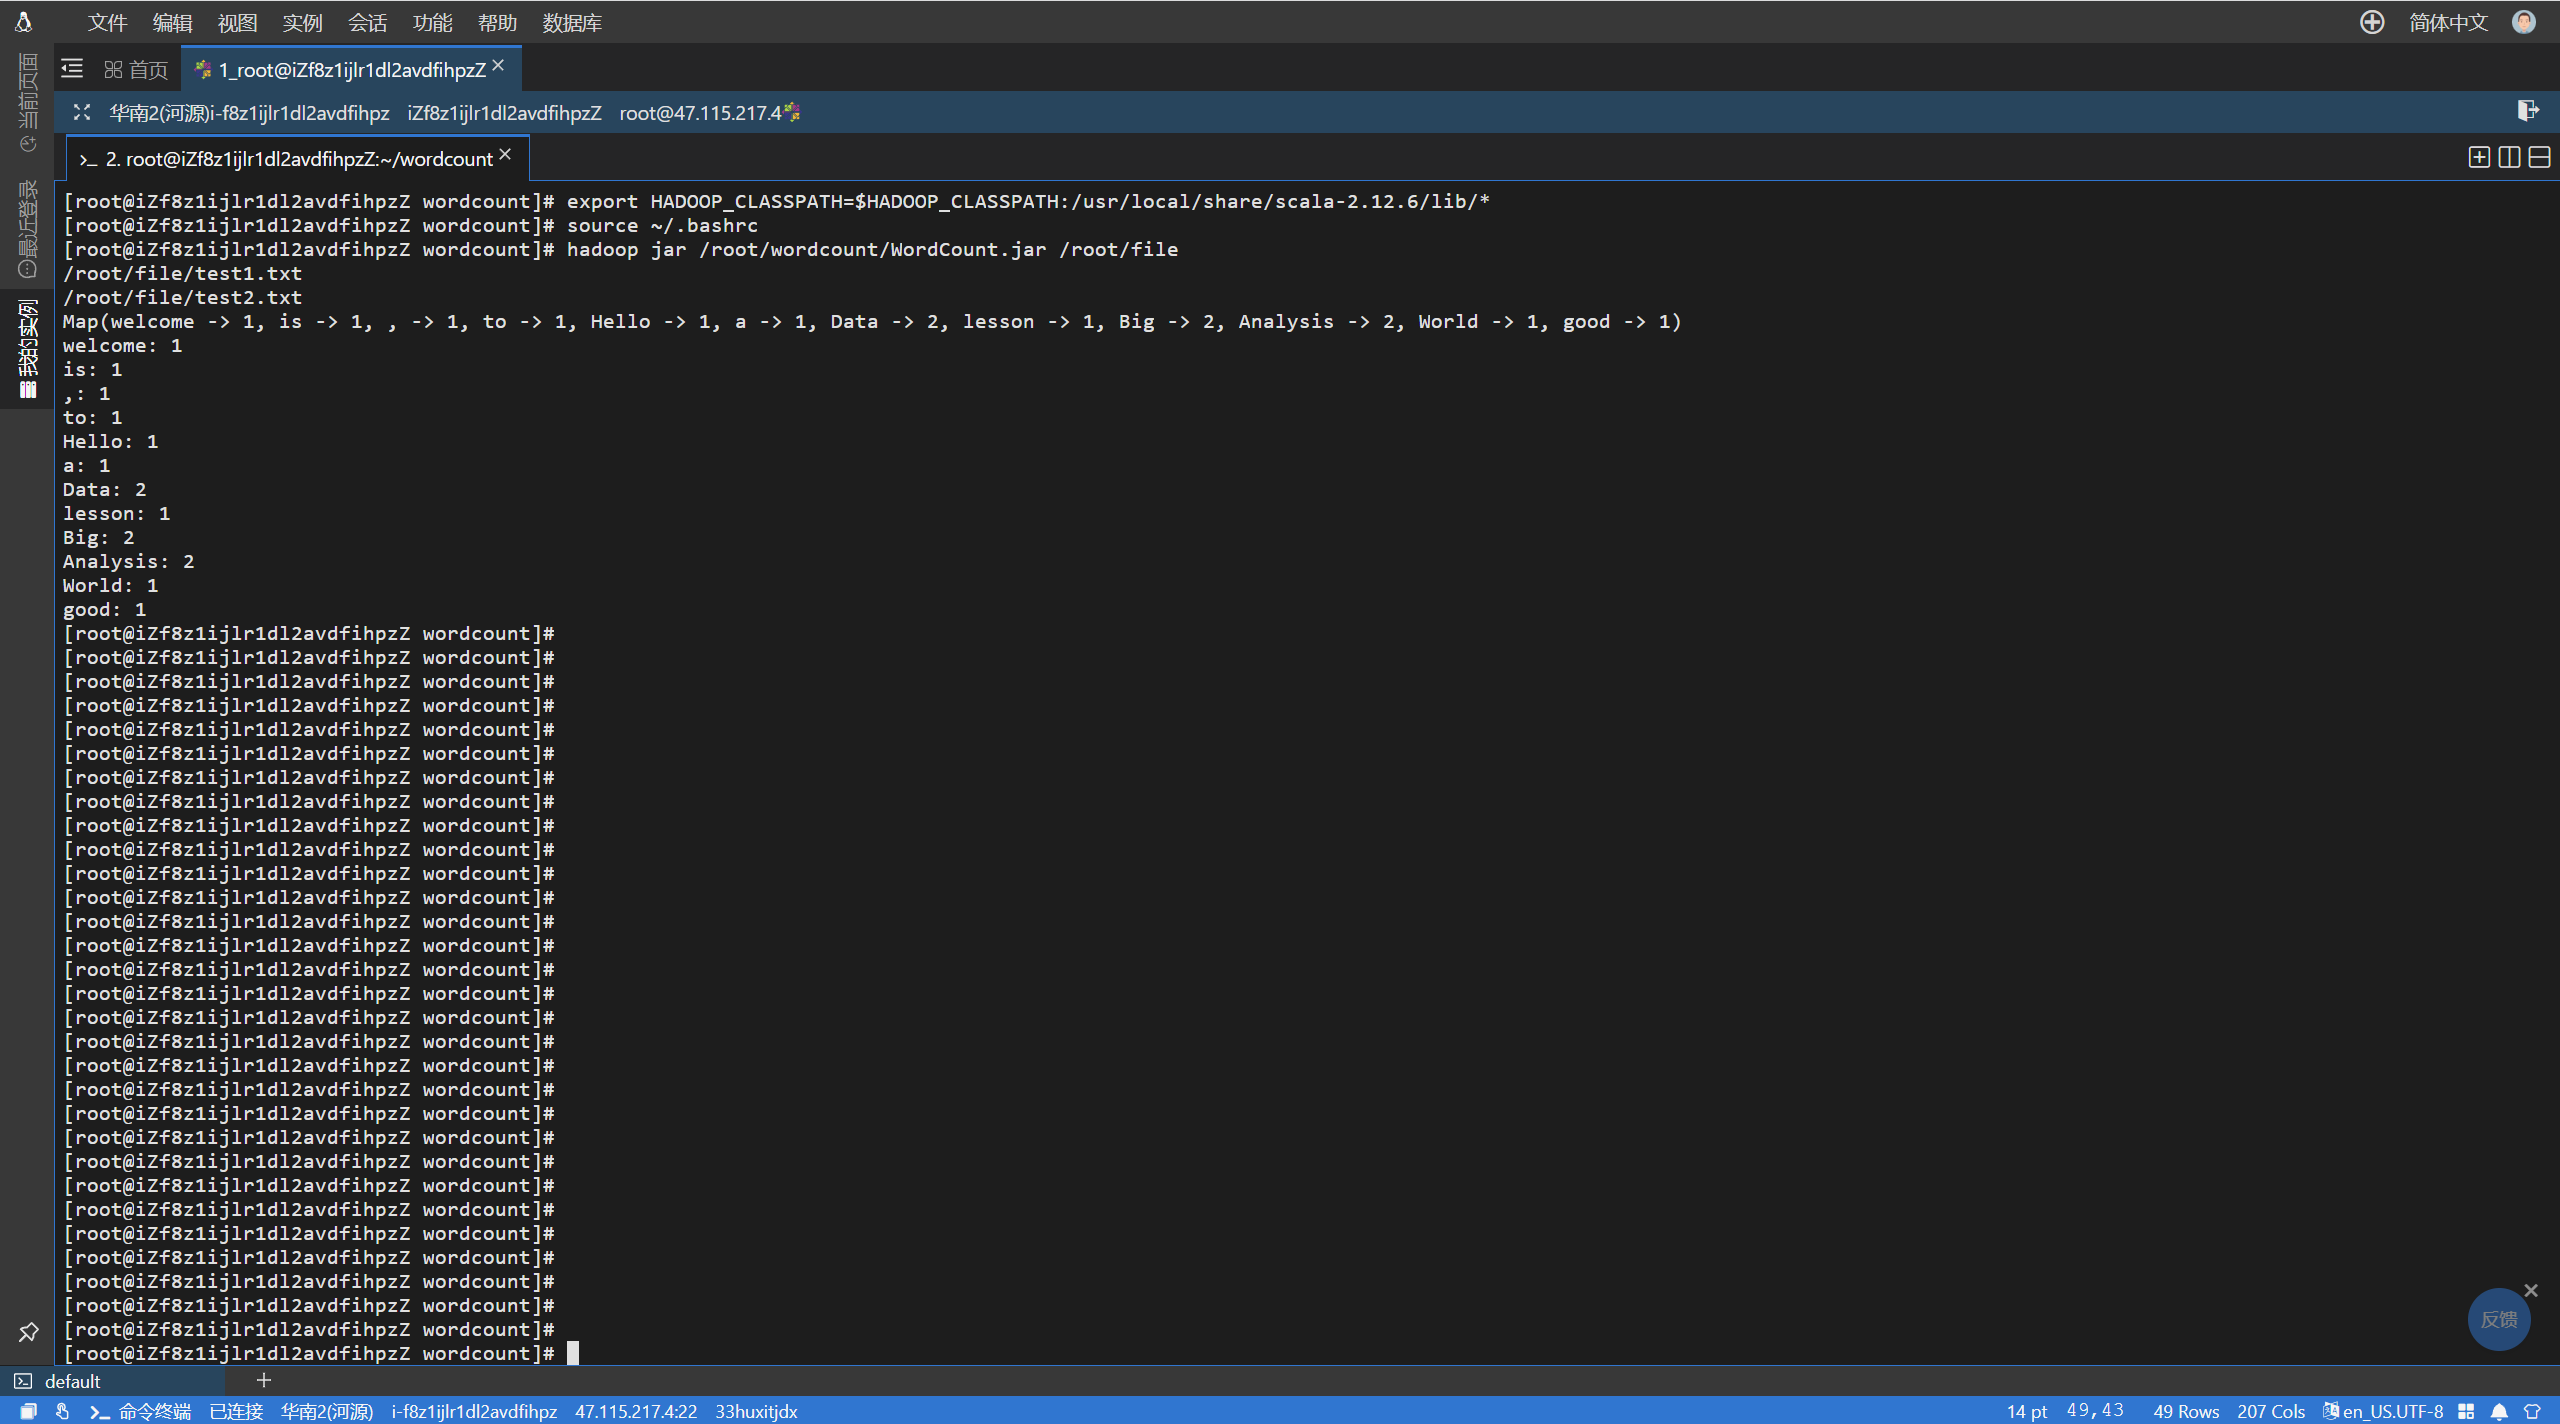
\includegraphics[width=10cm]{结果验证图.png}
        \caption{第二种方式在hadoop环境下,运行scala的wordcount}
        \label{i:a}
    \end{figure}
    \newpage
    \item 查看结果
    \begin{lstlisting}
hadoop fs -cat /output/part-r-00000
    \end{lstlisting}
    \begin{figure}[htp]
        \centering
        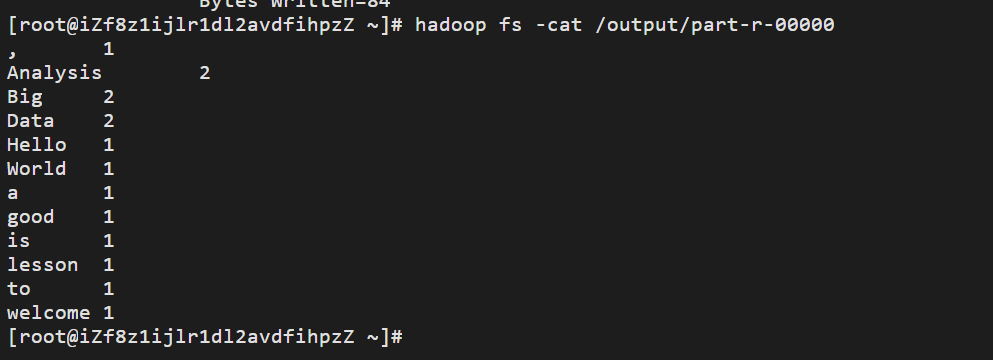
\includegraphics[width=10cm]{wordcount_result.png}
        \caption{统计test1文件和test2文件内所有单词的词频}
        \label{fig:a}
    \end{figure}
    \item 结果验证
    \par
    \begin{tabular}{|l|l|}
    \hline
    Word & Count \\
    \hline
    Analysis & 2 \\
    Big & 2 \\
    Data & 2 \\
    Hello & 1 \\
    World & 1 \\
    a & 1 \\
    good & 1 \\
    is & 1 \\
    lesson & 1 \\
    to & 1 \\
    welcome & 1 \\
    \hline
    \end{tabular}
    \par
    输出正确,程序运行正常
\end{enumerate}
\section{清理——终止实例服务}
在云服务器管理控制台停止用例
    \begin{figure}[htp]
        \centering
        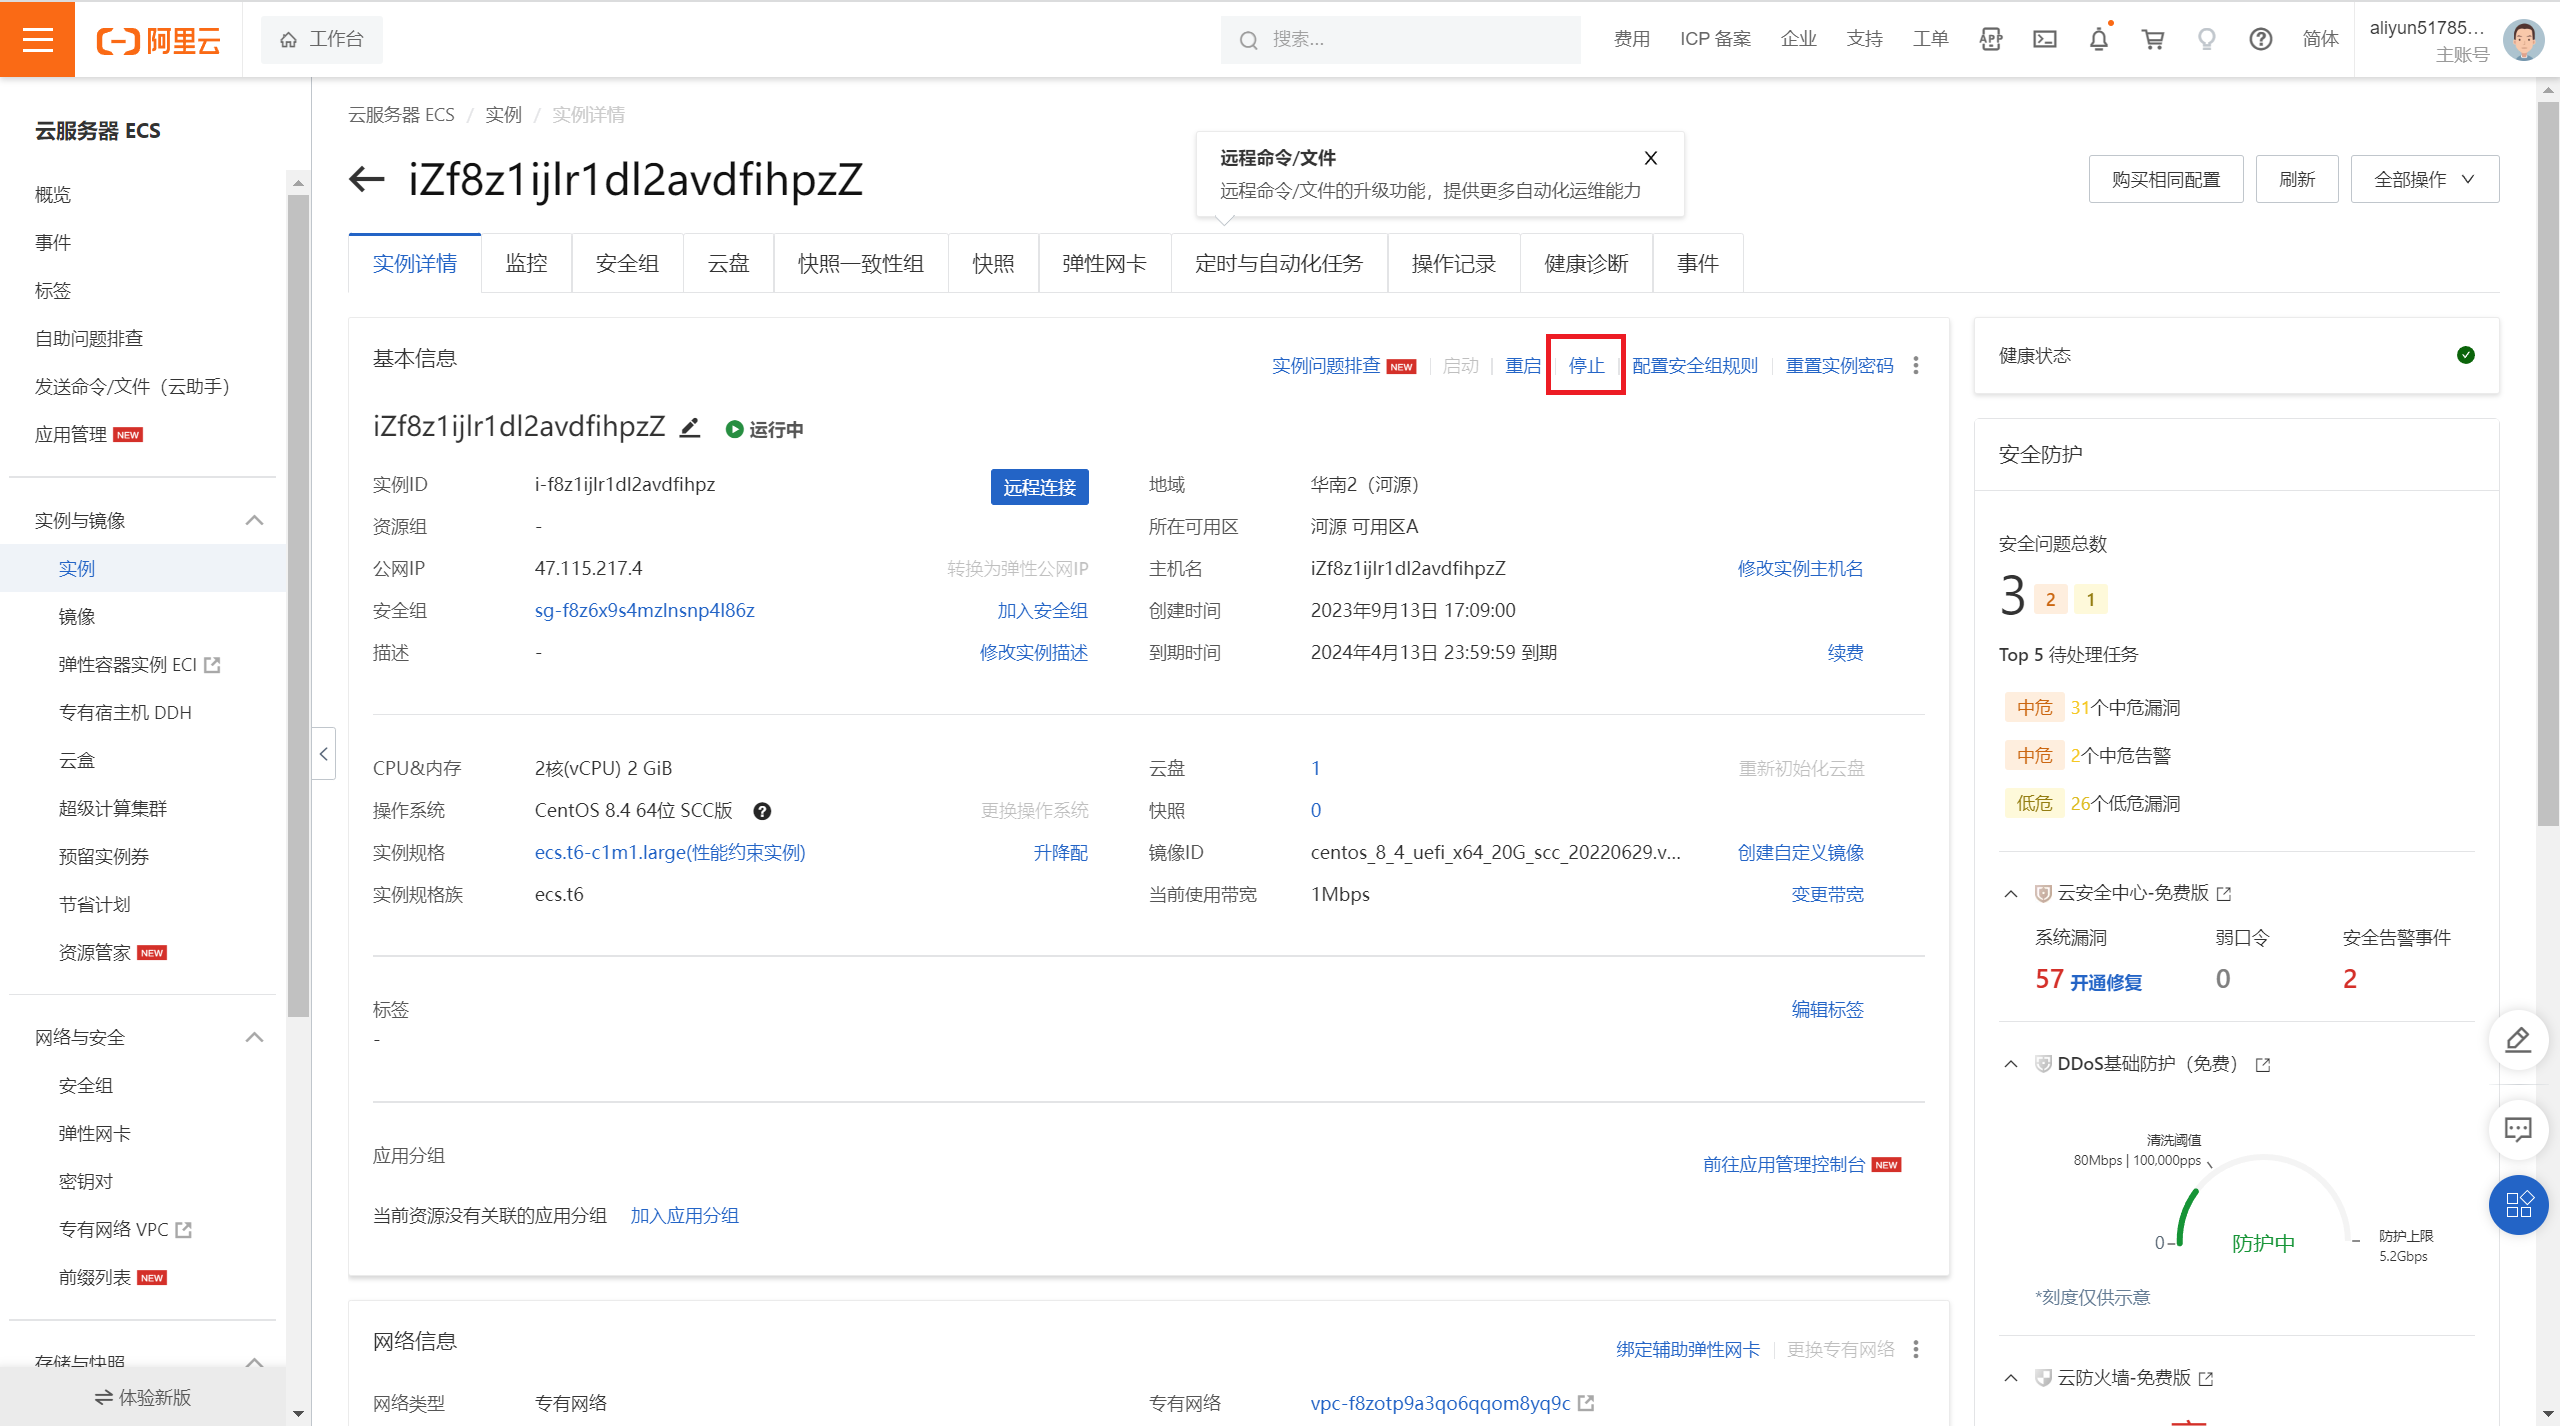
\includegraphics[width=10cm]{终止实例.png}
        \caption{终止实例}
        \label{fg:a}
    \end{figure}

\section{过程中的挑战及如何克服}
\begin{enumerate}
    \item 先需要找出哪个供应商有免费的学生服务,最后在阿里云中免费申请了7个月的云
    \item 不知道什么是bda环境,通过查询资料,最终选择hadoop作为作业的bda环境
    \item 配置环境是最复杂也是最繁琐的一项工程,因为我对这些东西一无所知,通过查询阿里云的官方文档已经搜索csdn和chatgpt,才最终配置好了hadoop、scala。
    \item 不懂如何在hadoop中运行scala代码,通过查询资料,渐渐明白了hadoop和scala的关系,将scala代码打包成jar,然后在Hadoop中运行。
\end{enumerate}
\end{document}
